\begin{figure*}[t]
 \begin{center}
  \begin{tabular}{m{6cm}m{6cm}}
   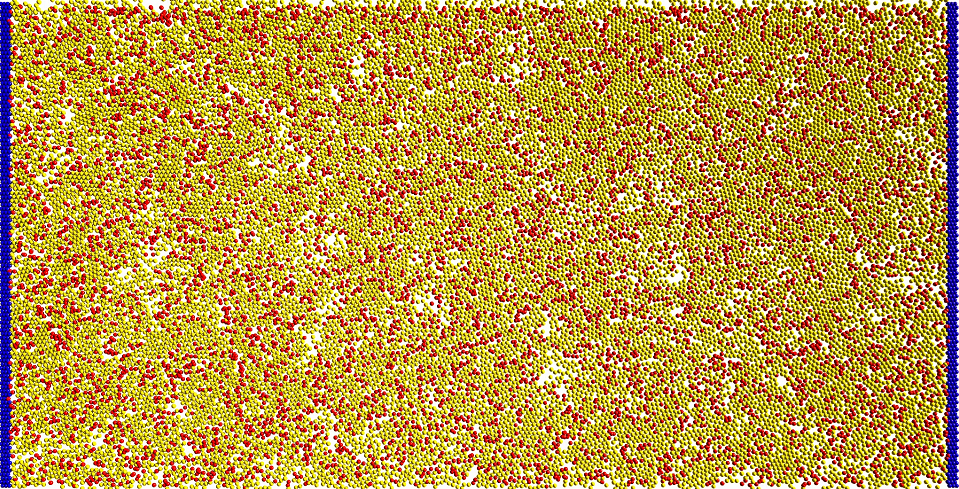
\includegraphics[width=5.9cm]{./figures/init_state.png} &
   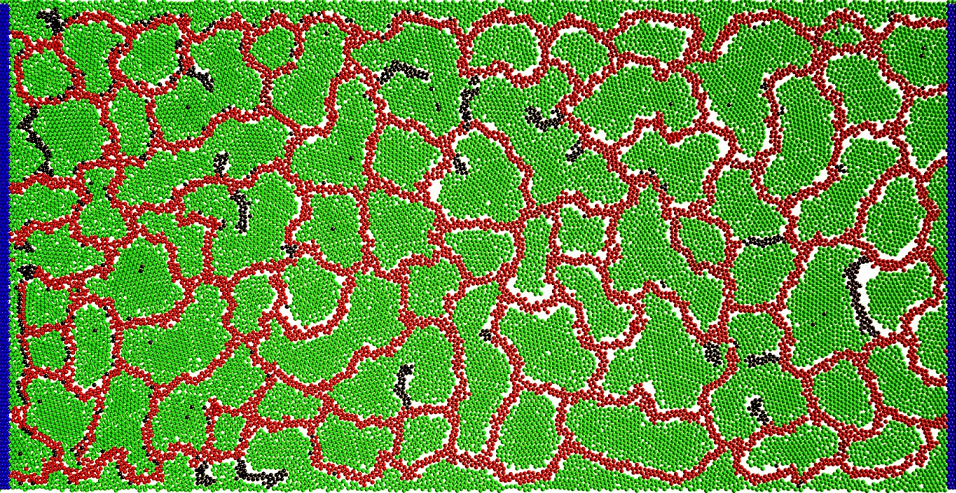
\includegraphics[width=5.9cm]{./figures/vessel30.png}\\
   (a) Initial random distribution & (b) Stable vascular network \\
   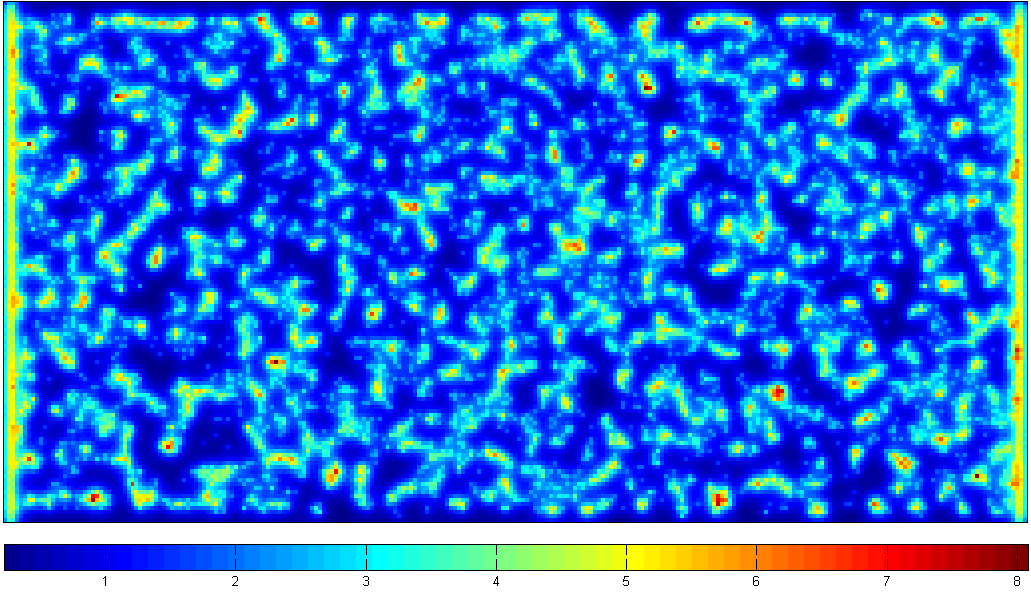
\includegraphics[width=5.9cm]{./figures/Chemo_init_state.png} \hspace{50mm} &
   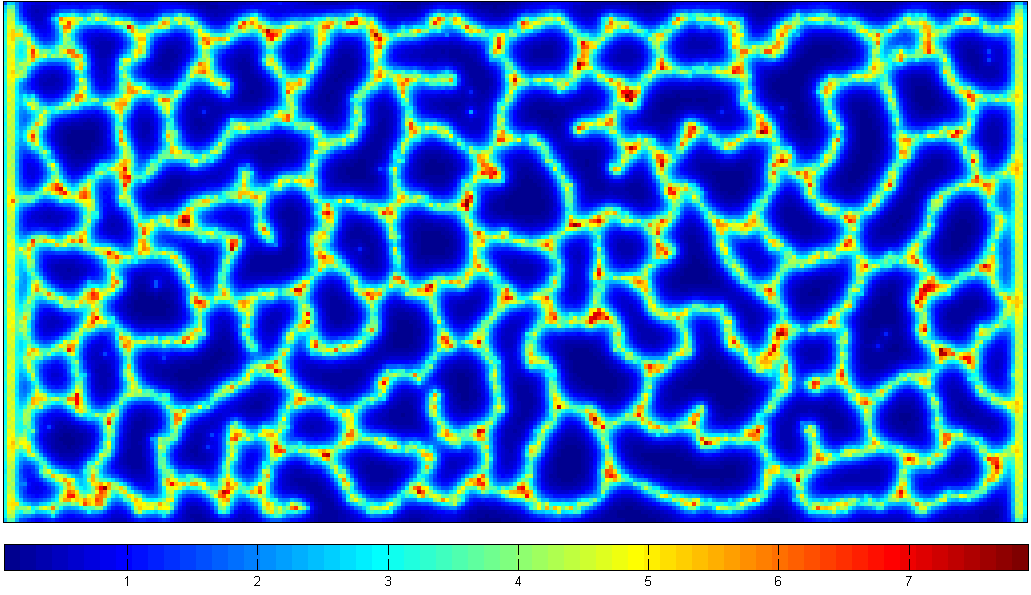
\includegraphics[width=5.9cm]{./figures/Chemo_steady_state.png} \hspace{50mm}\\
   (c) Chemoattractant during formation & (d) Chemoattractant state distribution \\
   \end{tabular}
   \end{center}
 \caption{\textbf{Self-organizing Network}: (a) is the initial conditions with fixed circulatory cells (blue) on each side and vascular (red) and supported cells (yellow) randomly mixed; (b) is the steady state network following self organization; (c) is the distribution of chemoattractant during vessel formation and (d) is at a steady state. In all images of biochemical distribution, blue signifies a low concentration, while red signifies a high concentration.}
 \vspace{+1mm}
\label{phaseOne}
\end{figure*} 